\documentclass[dvipdfmx,cjk,xcolor=dvipsnames,envcountsect,notheorems,12pt]{beamer}
% * 16:9 のスライドを作るときは、aspectratio=169 を documentclass のオプションに追加する
% * 印刷用の配布資料を作るときは handout を documentclass のオプションに追加する
%   (overlay が全て一つのスライドに出力される)

\usepackage{pxjahyper}% しおりの文字化け対策 (なくても良い)
\usepackage{amsmath,amssymb,amsfonts,amsthm,ascmac,cases,bm,pifont}
\usepackage{graphicx}
\usepackage[thicklines]{cancel}
\usepackage{url}
\usepackage{newtxmath}
\usepackage{bussproofs}

% スライドのテーマ
\usetheme{sumiilab}
% ベースになる色を指定できる
%\usecolortheme[named=Magenta]{structure}
% 数式の文字が細くて見難い時は serif の代わりに bold にしましょう
%\mathversion{bold}

%% ===============================================
%% スライドの表紙および PDF に表示される情報
%% ===============================================

%% 発表会の名前とか(省略可)
%\session{修論中間発表}
%% スライドのタイトル
\title{必要呼び高階関数型言語の\\コンパイラの形式的検証}
%% 必要ならば、サブタイトルも
%\subtitle{}
%% 発表者のお名前
\author{水野雅之}
%% 発表者の所属([] 内は短い名前)
%\institute[東北大学 住井・松田研]{工学部 電気情報物理工学科\\住井・松田研究室}% 学部生
\institute[東北大学 住井・松田研]{大学院情報科学研究科\\住井・松田研究室}% 院生
%% 発表する日
\date{2017年2月17日}

%% ===============================================
%% 自動挿入される目次ページの設定(削除しても可)
%% ===============================================

%% section の先頭に自動挿入される目次ページ(削除すると、表示されなくなる)
%\AtBeginSection[]{
%\begin{frame}
%  \frametitle{アウトライン}
%  \tableofcontents[sectionstyle=show/shaded,subsectionstyle=show/show/hide]
%\end{frame}}
%%% subsection の先頭に自動挿入される目次ページ(削除すると、表示されなくなる)
%\AtBeginSubsection[]{
%\begin{frame}
%  \frametitle{アウトライン}
%  \tableofcontents[sectionstyle=show/shaded,subsectionstyle=show/shaded/hide]
%\end{frame}}
%
%% 現在の section 以外を非表示にする場合は以下のようにする

%% \AtBeginSection[]{
%% \begin{frame}
%%   \frametitle{アウトライン}
%%   \tableofcontents[sectionstyle=show/hide,subsectionstyle=show/show/hide]
%% \end{frame}}
%% \AtBeginSubsection[]{
%% \begin{frame}
%%   \frametitle{アウトライン}
%%   \tableofcontents[sectionstyle=show/hide,subsectionstyle=show/shaded/hide]
%% \end{frame}}

%% ===============================================
%% 定理環境の設定
%% ===============================================

\setbeamertemplate{theorems}[numbered]% 定理環境に番号を付ける
\theoremstyle{definition}
\newtheorem{definition}{定義}
\newtheorem{axiom}{公理}
\newtheorem{theorem}{定理}
\newtheorem{lemma}{補題}
\newtheorem{corollary}{系}
\newtheorem{proposition}{命題}

%% ===============================================
%% ソースコードの設定
%% ===============================================

\usepackage{listings,jlisting}
%\usepackage[scale=0.9]{DejaVuSansMono}

\definecolor{DarkGreen}{rgb}{0,0.5,0}
% プログラミング言語と表示するフォント等の設定
\lstset{
  language={[Objective]Caml},% プログラミング言語
  basicstyle={\ttfamily\small},% ソースコードのテキストのスタイル
  keywordstyle={\bfseries},% 予約語等のキーワードのスタイル
  commentstyle={},% コメントのスタイル
  stringstyle={},% 文字列のスタイル
  frame=trlb,% ソースコードの枠線の設定 (none だと非表示)
  numbers=none,% 行番号の表示 (left だと左に表示)
  numberstyle={},% 行番号のスタイル
  xleftmargin=5pt,% 左余白
  xrightmargin=5pt,% 右余白
  keepspaces=true,% 空白を表示する
  mathescape,% $ で囲った部分を数式として表示する ($ がソースコード中で使えなくなるので注意)
  % 手動強調表示の設定
  moredelim=[is][\itshape]{@/}{/@},
  moredelim=[is][\color{red}]{@r\{}{\}@},
  moredelim=[is][\color{blue}]{@b\{}{\}@},
  moredelim=[is][\color{DarkGreen}]{@g\{}{\}@},
}

\newcommand{\keyword}[1]{\mathbf{#1}}
\newcommand{\LET}{\keyword{let}}
\newcommand{\IN}{\keyword{in}}

%% ===============================================
%% 本文
%% ===============================================
\begin{document}
\frame[plain]{\titlepage}% タイトルページ

\begin{frame}
	\frametitle{背景:コンパイラを形式的に検証する意義}
	\begin{center}
		\LARGE 
		\begin{columns}
			\begin{column}{0.75\textwidth}
				\begin{itembox}[c]{コンパイラのバグ}
					生成されるコードに影響\\
					デバッグが困難
				\end{itembox}
			\end{column}
		\end{columns}
		$\Downarrow$\\
		形式的検証が有用
	\end{center}
\end{frame}

\begin{frame}
	\frametitle{背景:コンパイラの形式的検証の既存研究}
	\begin{itemize}
		\item \alert{値呼び}$\cdot$高階関数あり
			\begin{itemize}
				\item CompCert [Leroy+ 2006]
					\begin{itemize}
						\item Cコンパイラ
					\end{itemize}
			\end{itemize}
		\item \alert{値呼び}$\cdot$高階関数なし
			\begin{itemize}
				\item Lambda Tamer [Chlipala 2007]
					\begin{itemize}
						\item 単純型付きλ計算のコンパイラ
					\end{itemize}
				\item CakeML [Kumar+ 2014]
					\begin{itemize}
						\item SMLのコンパイラ
					\end{itemize}
			\end{itemize}
	\end{itemize}
\end{frame}

\begin{frame}
	\frametitle{本研究の概要}
	\begin{itemize}
		\item 必要呼び高階関数型言語のコンパイラをCoqで検証
			\begin{itemize}
				\item De Buijnインデックスを採用
					\begin{itemize}
						\item 束縛の表現が簡潔に
					\end{itemize}
				\item 小ステップ意味論による定式化\mbox{[Ariola+ 1995]}を採用
					\begin{itemize}
						\item 束縛の対応を保つのが容易
					\end{itemize}
			\end{itemize}
	\end{itemize}
\end{frame}

\begin{frame}
	\frametitle{名前による束縛の表現の問題点}
	\begin{itemize}
		\item 項の等価性がCoqの等価性でなく\mbox{$\alpha$等価性}となる
			\[ \lambda x.\lambda y.x \overset{\alpha}{=} \lambda a.\lambda b.a \]
		\item Captureを避ける必要がある
			\only<1>{\[\begin{array}{l}
				[y \mapsto \alert{x}](\lambda x.y) \\
				\overset{\alpha}{\cancel{=}}~\lambda \alert{x}.\alert{x}
			\end{array}\]}
			\pause
			\[\begin{array}{l}
				[y \mapsto \alert{x}](\lambda x.y) \\
				\overset{\alpha}{=} \lambda z.\alert{x}
			\end{array}\]
	\end{itemize}
\end{frame}

\begin{frame}
	\frametitle{De Bruijnインデックスによる束縛の表現}
	\begin{itemize}
		\item 内側から数えて何番目の束縛かで表現
			{\LARGE \[\begin{array}{lcl}
				\lambda x.x~(\lambda y.x~y) & \Rightarrow & \lambda.0~(\lambda.1~0)
			\end{array}\]}
		\item $\alpha$等価な式は文面上も同じ
			{\LARGE \[\begin{array}{lcl}
				\lambda x.\lambda y.x & \Rightarrow & \lambda.\lambda.1 \\
				\lambda a.\lambda b.a & \Rightarrow & \lambda.\lambda.1 \\
			\end{array}\]}
	\end{itemize}
\end{frame}

\begin{frame}
	\frametitle{必要呼び高階関数型言語の操作的意味論}
	\begin{itemize}
		\item 抽象機械によるもの
			\begin{itemize}
				\item STG machine [Jones 1992]
			\end{itemize}
		\item 対象言語の構文でヒープを表現
			\begin{itemize}
				\item 大ステップ意味論を採用
					\begin{itemize}
						\item \mbox{[Launchbury 1993]}
					\end{itemize}
				\item 小ステップ意味論を採用
					\begin{itemize}
						\item \mbox{[Ariola+ 1995]}
					\end{itemize}
			\end{itemize}
	\end{itemize}
	\begin{flushright}
		\Large $\Rightarrow$自明ではない
	\end{flushright}
\end{frame}

\begin{frame}
	\frametitle{大ステップ意味論による表現[Launchbury 1993]}
	\begin{itemize}
		\item サンクのポインタを変数で表現
	\end{itemize}
%
	\Large
	\fbox{$H ; t \Downarrow H' ; v$}
	\begin{prooftree}
		\AxiomC{$(x\mapsto t_1, H) ; t_2 \Downarrow H' ; v$}
		\UnaryInfC{$H ; (\LET~x=t_1~\IN~t_2) \Downarrow H' ; v$}
	\end{prooftree}
	\begin{prooftree}
		\AxiomC{$H_2 ; t \Downarrow H_2' ; v$}
		\UnaryInfC{$(H_1, x\mapsto t, H_2) ; x \Downarrow (H_1,x\mapsto v, H_2') ; v$}
	\end{prooftree}
\end{frame}

\begin{frame}
	\frametitle{評価の導出例[Launchbury 1993]}
	\normalsize
	\begin{prooftree}
		\AxiomC{$\varnothing ; 1 \Downarrow \varnothing ; 1$}
		\UnaryInfC{$(z \mapsto 1) ; z \Downarrow (z \mapsto 1) ; 1$}
		\UnaryInfC{$\varnothing ; \LET~z=1~\IN~z \Downarrow (z \mapsto 1) ; 1$}
		\UnaryInfC{$(x \mapsto y, y \mapsto \LET~z=1~\IN~z) ; y \Downarrow (x \mapsto y, y \mapsto 1, z \mapsto 1) ; 1$}
	\end{prooftree}
%
	\pause
	\begin{itemize}
		\item ヒープ内の式も自由変数をもつ
		\item 評価中にヒープの要素が増える
			\begin{itemize}
				\item 大ステップ意味論なので何個増えるか分からない
			\end{itemize}
	\end{itemize}
	\pause
	\begin{flushright}
		\Large $\Rightarrow $De Bruijn indexで束縛の対応を保ち\\にくい
	\end{flushright}
\end{frame}

\begin{frame}
	\frametitle{小ステップ意味論による表現[Ariola+ 1995]}
	{\large 
		\[\begin{array}{lcl}
			v & ::= & \lambda x.t \\
			a & ::= & v~|~\LET~x=t~\IN~a \\
		\end{array}\]
%
		\fbox{$t \longrightarrow t'$}
		\[\begin{array}{lcl}
			\LET~x=v~\IN~E[x] & \longrightarrow & \LET~x=v~\IN~E[v] \\
			(\LET~x=t_1~\IN~a)~t_2 & \longrightarrow & \LET~x=t_1~\IN~a~t_2 \\
		\end{array}\]}
	\begin{itemize}
		\item 評価文脈を活用
		\item 簡約で位置が入れ替わる束縛の数は一定
	\end{itemize}
	\begin{flushright}
		\Large $\Rightarrow $De Bruijn indexでも束縛の対応を保てる
	\end{flushright}
\end{frame}

\begin{frame}
	\frametitle{Coqによる定式化(1/2)}
	\begin{figure}
		\centering
		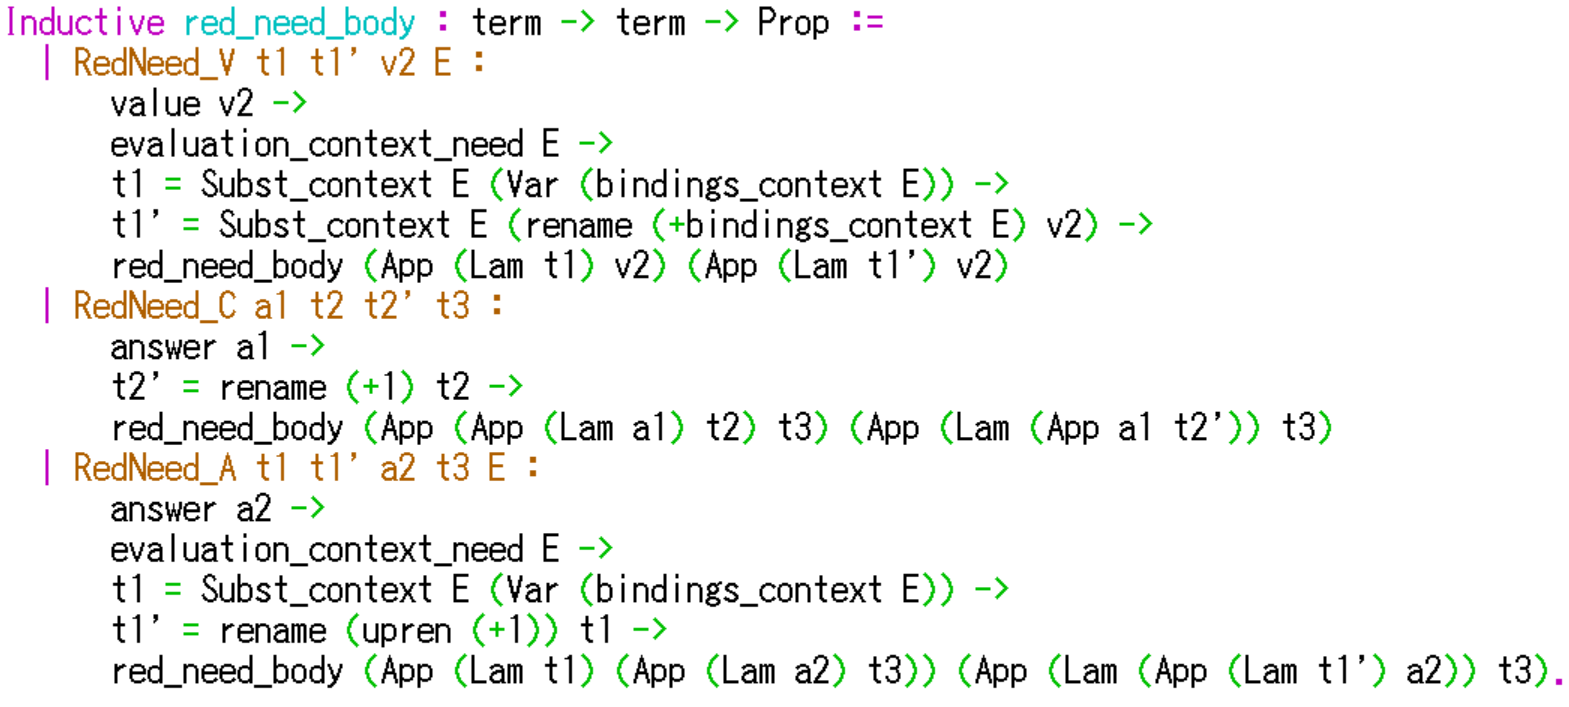
\includegraphics[width=\textwidth]{./red_def.png}
	\end{figure}
\end{frame}

\begin{frame}
	\frametitle{Coqによる定式化(2/2)}
	\begin{figure}
		\centering
		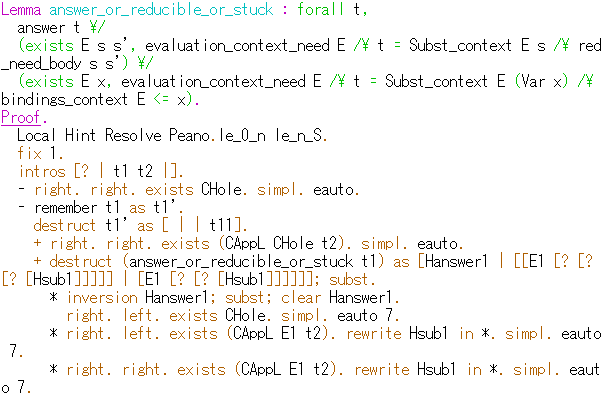
\includegraphics[width=\textwidth]{./red_det.png}
	\end{figure}
\end{frame}

\begin{frame}
	\frametitle{まとめ}
	\begin{itemize}
		\item 必要呼び高階関数型言語の意味をCoqで定式化できた
			\begin{itemize}
				\item De Bruijn indexを必要呼びにも適用、束縛の取り扱いを簡単化
				\item 簡約の決定性程度は証明済
					\begin{itemize}
						\item Ariolaらの意味論のside conditionの欠如を発見
					\end{itemize}
			\end{itemize}
		\item 必要呼び高階関数型言語のコンパイラをCoqで検証
			\begin{itemize}
				\item 短期的には名前呼びとの対応を証明
			\end{itemize}
	\end{itemize}
\end{frame}

\end{document}

